\subsection{Steuerung}
\mysubsubsection{Fabian Gärtner}{Physikalische Steuerung} \label{Marker}

\begin{figure}[!htbp]%[htbp]
	\centering
		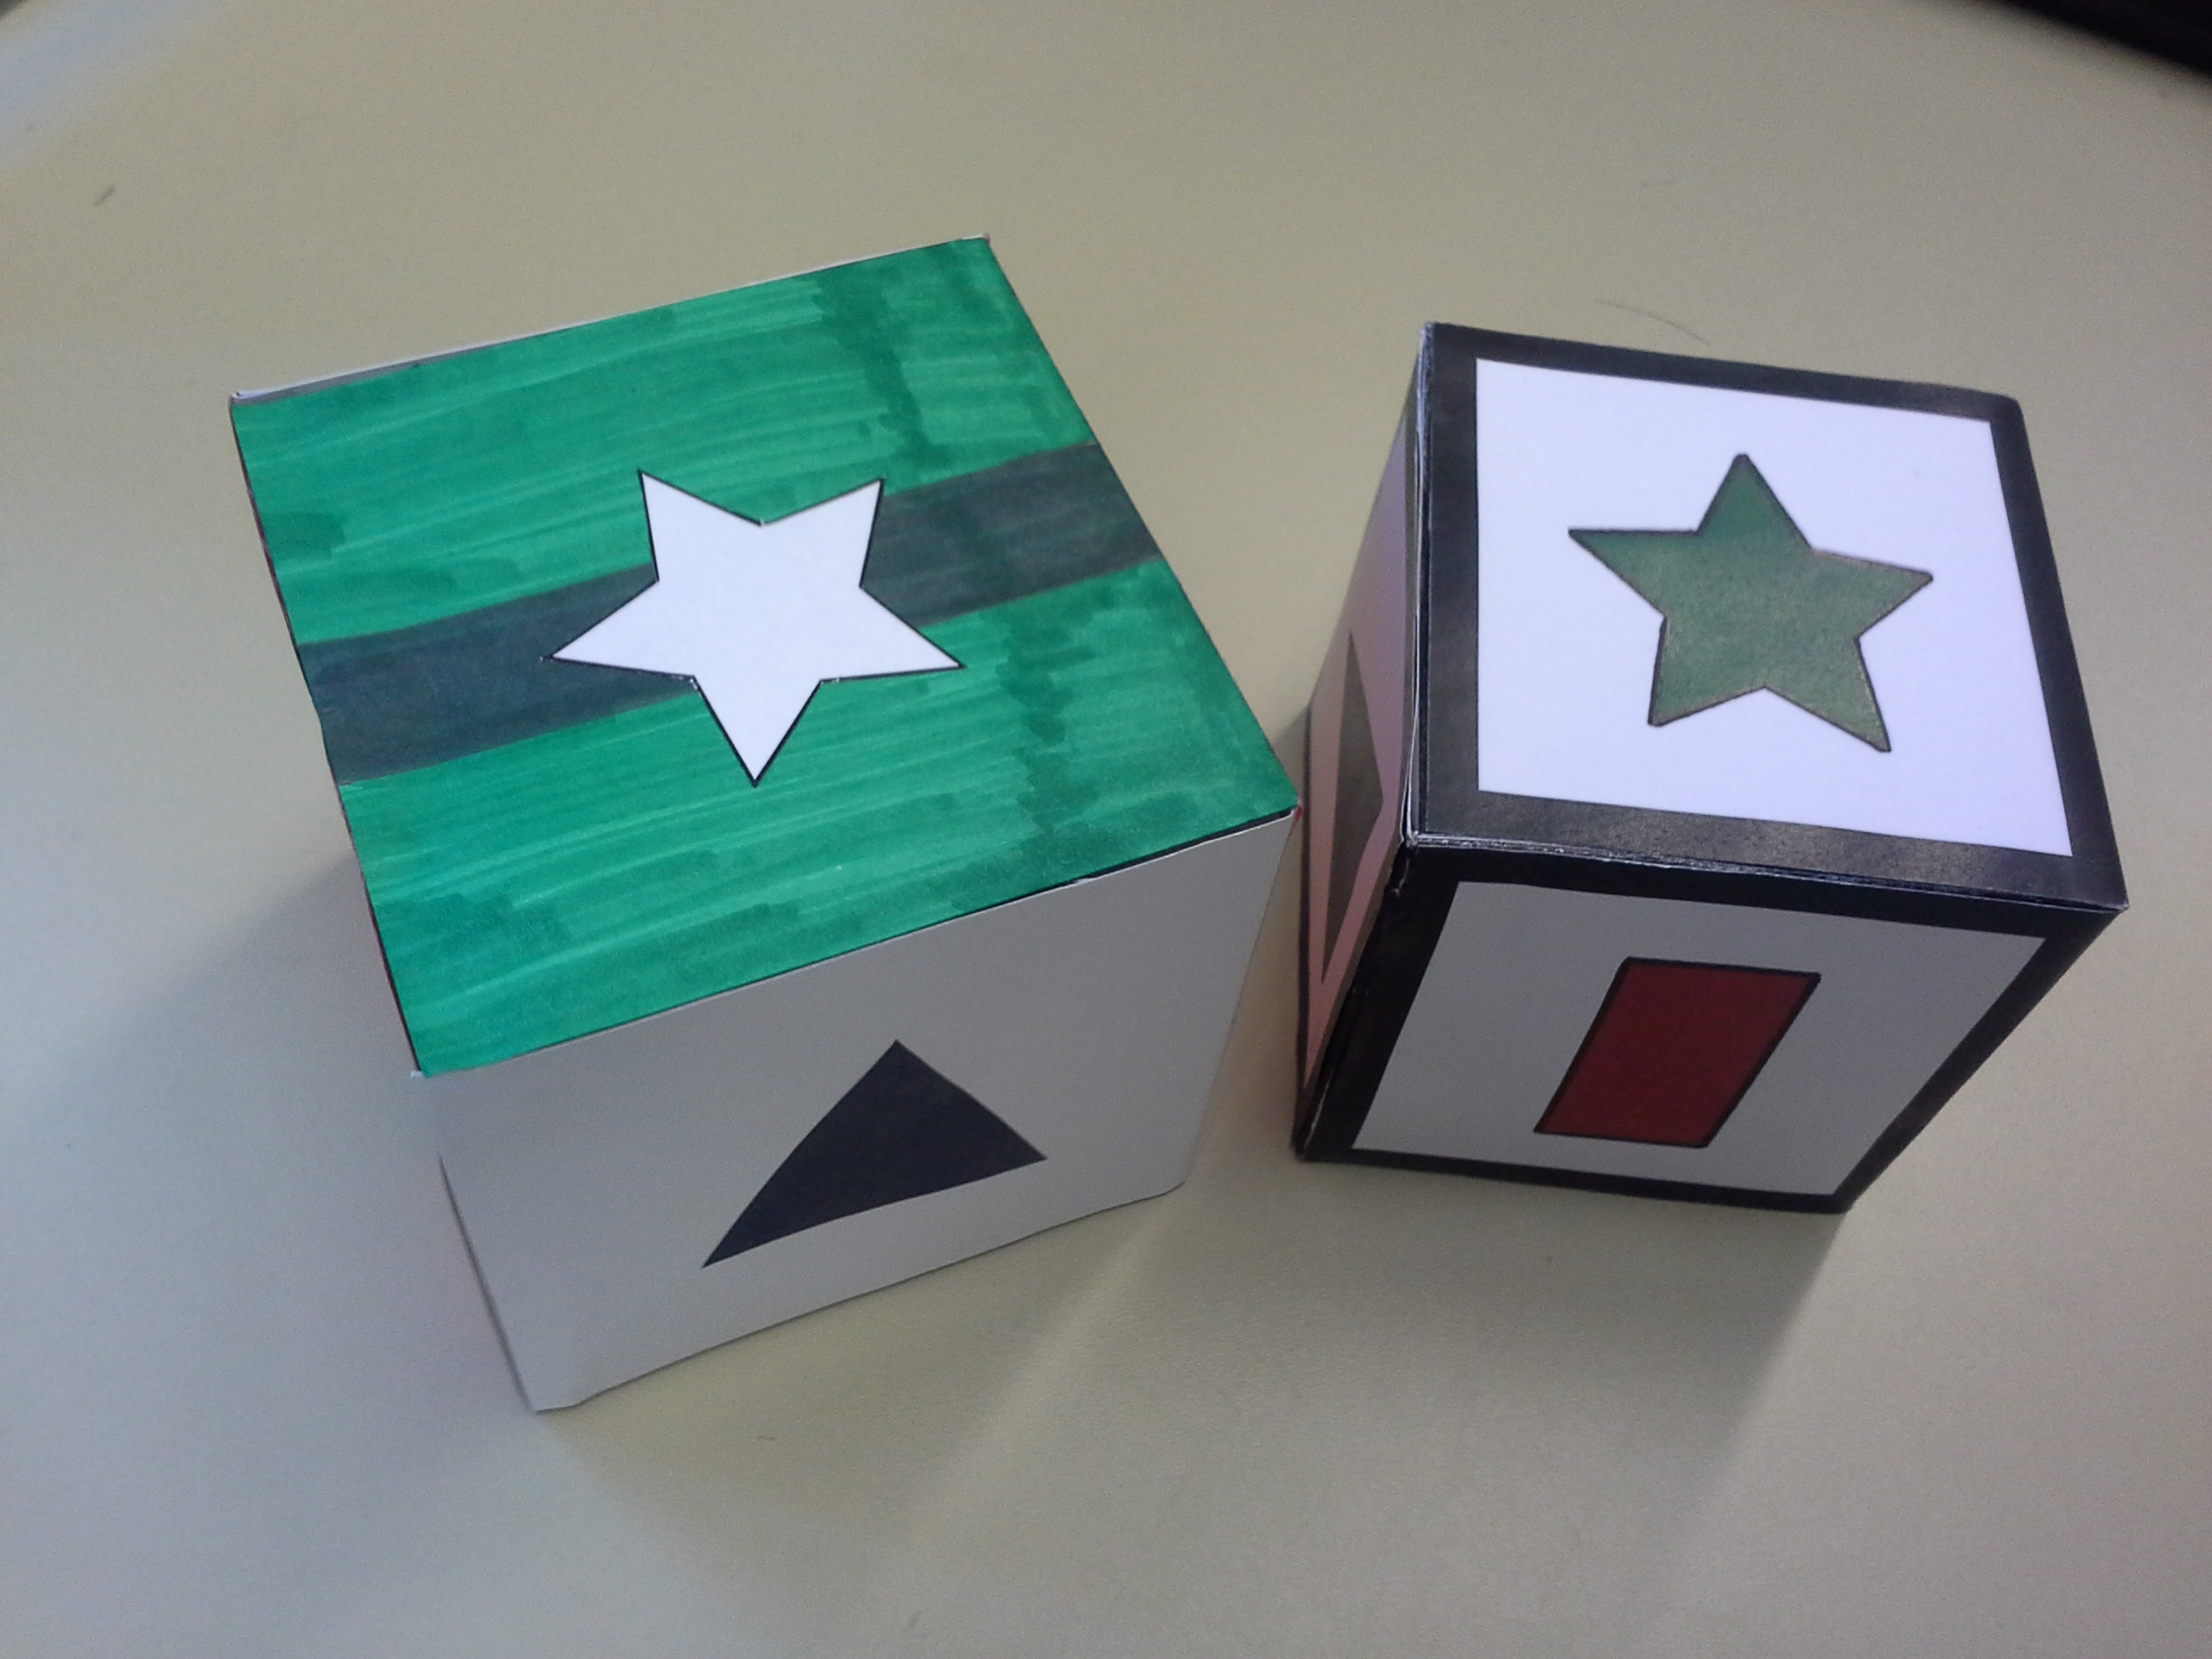
\includegraphics[width=1.0\textwidth]{images/wuerfel}
	\caption{Markerwürfel in verschiedenen Stadien}
	\label{fig:Wuerfel}
\end{figure}

Da die Steuerung für den Spieler so einfach wie möglich gehalten werden soll, sodass auch Personen, die bisher nicht mit Videospielen und der entsprechenden Peripherie (also bspw. Controller) vertraut sind, inCubed spielen können, ist jegliche Interaktion mit dem Spiel durch Blickkontakt mit Interaktionspunkten möglich. Es ist allerdings, sei es aus Platzmangel oder aus gesundheitlichen Gründen, nicht immer möglich, sich vollständig nach hinten, oben oder unten umzusehen, was die Erkundung der Welt einschränken und damit das Lösen der Rätsel erschweren würde. Die Verwendung eines handelsüblichen Controllers zur Bewegung der Spielwelt wäre hier aber nicht sinnvoll, da dieser mit seiner Vielzahl an Tasten vor allem von ungeübten Spielern eher unintuitiv zu bedienen wäre, vor allem da durch Verwendung der VR-Brille der Controller nicht sichtbar ist. Daher steht für inCubed ein deutlich intuitiverer und unkonventioneller Controller in Form eines Würfels zur Verfügung, der sich sowohl in die Rahmenhandlung einfügt, als auch dem Spieler auf einfache Art und Weise ermöglicht, sich in der Welt umzusehen. Dazu muss er während des Spiels lediglich diesen Würfel vor die Kamera des Smartphones, das sich zwar in der VR-Brille befindet, aber durch das Sichtfenster in der VR-One die Umgebung filmen kann, halten und bei Bedarf so drehen, dass eine der sechs Würfelseiten zur Kamera zeigt. Dies führt gleichzeitig dazu, dass sich die Spielwelt entsprechend um jeweils 90° dreht und so auch andere Teile der Welt erkundet werden können, ohne dass sich der Spieler selbst umdrehen muss.

Das Design dieses Würfels, auf dessen sechs Seiten sich sechs unterschiedliche Formen (Dreieck, Stern, Rechteck, Kreis, Pentagon und Heptagon) befinden, wurde so gewählt, dass zum einen die Bewegung des Würfels durch die Kamera des Smartphones möglichst effizient und zuverlässig erkannt werden kann (mehr zum technischen Hintergrund in den späteren Kapiteln) und zum anderen so, dass er optimal zur Thematik von inCubed passt. Die Geschichte in inCubed erklärt, dass es sich bei diesem Würfel um den Hilferuf des verrückten Wissenschaftlers handelt. Da der Wissenschaftler von geometrischen Formen besessen scheint, hat er nicht nur den \enquote{Remote Cube} sondern auch diese SOS-Maschine in Form eines Würfels gebaut und mit simplen mathematischen Strukturen versehen. Da im Spiel gegenüberliegende Welten konträr sind, sind auch diese Formen auf gegenüberliegenden Seiten des Würfels so unterschiedlich wie möglich (bspw. das Dreieck mit seinen drei Eckpunkten und der Kreis, der technisch gesehen aus einer Vielzahl an Eckpunkten besteht). Sie haben aber dennoch die gleiche Farbe, da sie wie die gegenüberliegenden Welten im Spiel zusammengehören. Besonders am Ende des Spiels, nach Absetzen der Brille, wird dem Spieler dann auch bewusst, dass sein Controller starke Ähnlichkeit mit der Maschine hat, die durch das Lösen der Rätsel wieder zusammengesetzt werden musste.

\mysubsubsection{Alexander Scheurer}{Blick Steuerung}

Als weitere intuitive Steuermethode, um sich in der Welt von inCubed zu bewegen, ist eine Steuerung über das Anblicken von Weg- bzw. Aktionspunkten eingebaut. Blickt man einen solchen Punkt eine gewisse Zeit an, so wird die damit verbundene Aktion, z.B. Aufsammeln des Gegenstands oder Reise an den entsprechenden Punkt, ausgeführt.

Wegpunkte werden im Spiel als grüne Sphären dargestellt. Aktionspunkte befinden sich auf mehr oder weniger auffälligen Objekten, was den Wimmelspielcharakter des Spiel ausmacht.

Prototypentests haben ergeben, dass ein Zeitraum von ca. 2 Sekunden als passend empfunden wird um Aktionen auszulösen. Ein längerer Zeitraum führt dazu, dass der Spieler zu schnell einen Punkt als nicht relevant verwirft, bei einem kürzeren kommt es zu zufälligen Funden.

\mysubsubsection{Alexander Scheurer}{Trigger und Aktionen}

Anhand von zwei Prototypen wurde das Verhalten und die Anforderungen von Triggern für Weg- und Aktionspunkte getestet.

Eine Komponente um beide Arten zu realisieren ist ein Rayemitter, der sich am Kopfteil des Kamerarigs befindet und somit immer in die Kopfrichtung des Spielers zeigt. Der Raycast 'triggert' im Falle des Auftreffens auf ein entsprechendes Objekt die jeweilige Aktion.

Im Fall eines Wegpunkts wird die Reise dorthin gestartet. Der Spieler hat während der Reise immer noch die Kontrolle über die Rotation und Neigung der Kamera. Der Prototyp wurde auch dazu verwendet, entsprechende Ease-In und Ease-Out Methoden zu testen, um das Bewegungsgefühl so angenehm wie möglich zu machen.
Die Entscheidung ist zwischen Potenz-, Winkel-, Exponentialfunktionen auf die sogenannte Smoothstep-Funktion gefallen.

Aktionspunkte haben mehrere Fähigkeiten und können über den Unity-Inspector angepasst werden. Es können beliebig viele Gamestates geändert, das Gameobjekt zerstört, beliebige Prefabs instantiiert oder/und für komplexere Operationen eine Funktion in einem Event-Controller aufgerufen werden. Der Event-Controller ist hier die Sammlung angepasster Funktionen die speziell für einige wenige Trigger geschrieben werden.

Ebenfalls können beide Triggerarten von beliebig vielen Gamestats abhängig sein.
